%!TEX root = ../thesis.tex
\chapter{Ohua}

\label{ch:Ohua}

Ohua\cite{Ertel:2015:OID:2807426.2807431}\cite{Ohua:library:link} is parallelisation framework implemented in Java\cite{JavaLanguage} and Clojure\cite{ClojureLanguage}.

At compile time Ohua transforms the program into a dataflow graph, see Figure~\ref{fig:ohua-compiler-flow}.
The program itself is written in a Clojure EDSL, input in the lower part of Figure~\ref{fig:ohua-compiler-flow} and composes of so called ``stateful functions''\ref{sec:stateful-functions}, input in the upper part of Figure~\ref{fig:ohua-compiler-flow}.

\begin{figure}
  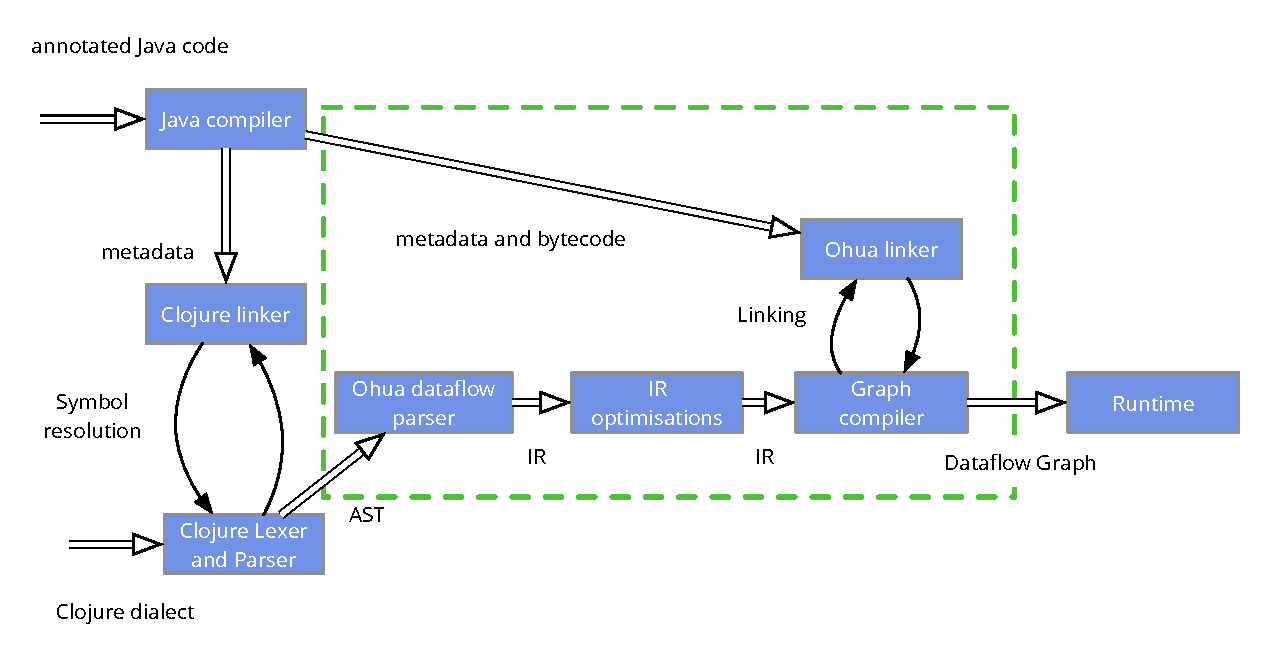
\includegraphics[width=\textwidth]{../Figures/ohua-compiler-flow}
  \caption{Compiler flow of Ohua}
  \label{fig:ohua-compiler-flow}
\end{figure}


The created dataflow graph is a representation of atomic parts of the program, the stateful functions, and the data dependencies between them.
Since Ohua currently does not support recursion this graph is a DAG.
Nodes are call sites of atomic pieces of code, these pieces of code are called stateful functions.
Edges represent data dependencies between the call sites.
Edge direction indicates result and argument.
The result of the source node is argument to the target node.
The result value of one node may be used by multiple other nodes and each node can have multiple inputs or none at all.
An example of how this transformation looks can be seen in Figure~\ref{fig:ohua-code-example}.
All of the called functions here, such as \texttt{vector}, \texttt{add} etc. have to be implemented as stateful functions, see Figure~\ref{fig:ohua-sfn-example}.

\begin{figure}[h]
  \begin{subfigure}{.5\textwidth}
\begin{minted}{Clojure}
(def main
  (ohua
    (let [a (increment 1)
          b (add 2 a)
          c (some-action)]
      (vector a b c))))
\end{minted}
  \end{subfigure}
  \begin{subfigure}{.5\textwidth}
    \includegr{ohua-code-example}    
  \end{subfigure}

\caption{An example for code transformation in Ohua}
\label{fig:ohua-code-example}
\end{figure}

\begin{figure}[h]
\begin{minted}{Java}
public class Add {
  @defsfn // <- the annotation to make a stateful function
  public Int add(int i1, int i2) {
    return i1 + i2;
  }
}
\end{minted}
\caption{Example implementation for \texttt{add}}
\label{fig:ohua-sfn-example}
\end{figure}

This dataflow graph can then be executed by a dataflow execution runtime which dynamically schedules the nodes of the graph.
The runtime knows about the data dependencies between the nodes of the graph and therefore can schedule independent nodes in parallel.
Data independent nodes can be executed in parallel.
Also subsequent calls to the same node with unrelated data, as a result of a mapping operation for instance, can be executed in parallel.
This property allows us to do deterministic state modifications on an object of the class the stateful function is attached to.
As a result we obtain pipeline parallelism.

\section{Stateful Functions}

\label{sec:stateful-functions}

Stateful functions are the implementation for the nodes of the Ohua dataflow graph.
They represent atomic pieces of code which the Ohua runtime schedules.
Stateful functions can be implemented in Java or Scala\cite{ScalaLanguage} by annotating a method with \texttt{@defsfn}, or in Clojure by using the \texttt{defsfn} macro.
Each stateful function has an associated class, which holds an internal, opaque state of the node.
Whenever a stateful function is referenced in code the runtime creates a new instance of the class in which the stateful function is implemented.
As a result invocations at the same call site of a stateful function implicitly share an opaque state.
But different call sites do not share state implicitly.
To share state across call sites the state has to be explicitly passed to the function as an argument.
This ensures that state sharing is transparent to the runtime without requiring in depth knowledge about the structure of the state itself or the stateful function.

When executing the dataflow graph the runtime dynamically schedules nodes on a configurable number of cpu cores.
As a result the precise order in which the graph is executed is indeterministic.
However the runtime ensures that for each node the order of its subsequent invocations is preserved which ensures correct semantics not only in the high level algorithm but also with regards to the internal, opaque state of each stateful function itself.

\section{Algorithms}

Algorithms express high level, parallelisable computations in Ohua.
These algorithms are written in Ohua's Clojure EDSL using the \texttt{algo} macro.
Algorithms use and combine stateful functions to express complex computations.
Algorithms are generally assumed to be pure in so far as there are no data dependencies between any two functions which are not directly visible via function arguments and return values.
No two functions should share data in any way other then by explicitly passing them from one to the other via arguments and result.
Furthermore there should not be any dependency on invocation ordering which is not expressed directly through data dependencies.
The snippet of code in Figure~\ref{fig:indeterministic-code} for example: If this were normal Clojure code, the read would be executed before the write due to the sequential, deterministic semantics of a Clojure \texttt{let} binding.
In Ohua however, since there are no data dependencies between \texttt{read} and \texttt{write}, the execution order of those two stateful functions is nondeterministic and they could even be executed simultaneously.
The graph in Figure~\ref{fig:indeterministic-code} shows very nicely how at this stage there is no visible order for those two actions in the compiled graph.
Both \texttt{read-database > write-database > compute}\footnote{\texttt{a > b} means \texttt{a} is executed before \texttt{b}} and \texttt{write-database > read-database > compute} are valid topological orderings of the dataflow graph and Ohua only guarantees \emph{a} topological call order, not which.
When the algorithm is executed using the \texttt{ohua} or \texttt{<-ohua} macro the algorithms Clojure code is compiled into a dataflow graph and executed by the Ohua runtime.

\begin{figure}
  \begin{subfigure}{0.5\textwidth}
\begingroup
\definecolor{green(html/cssgreen)}{rgb}{0.0, 0.5, 0.0}
\catcode`\@=\active
\def@#1@{\textcolor{green(html/cssgreen)}{#1}}
\begin{minted}[escapeinside=||]{Clojure}
(|@defalgo@| my-algo []
  (let [a (read-database)
        b (write-database)]
    (compute a b)))
\end{minted}
\endgroup
  \end{subfigure}
  \begin{subfigure}{0.5\textwidth}
    \includegr{indeterministic-code-example}
  \end{subfigure}
\caption{An example of indeterministic code}
\label{fig:indeterministic-code}
\end{figure}

\section{Dataflow IR}

Ohua was already using a data flow graph for its runtime execution model, but in order to implement Yauhau we also needed a (much simpler) compile time data flow graph representation.
A simplified dataflow representation also lends itself nicely for performing high level optimisations on the graph itself as well as perform analysis such as type checking\footnote{This may be subject of future work}.
As a result the dataflow IR on which \yauhau{} operates is now directly part of Ohua and its compilation pipeline.

Like the final dataflow graph the IR encodes the dataflow relationships inside of the program.
The description of the graph contains two elements:

\begin{enumerate}
    \item \textbf{Bindings} are named data elements or alternatively can be interpreted as a data path.
    Each binding has to be unique and constant, which means it can only be assigned once, in which case we also speak of the \textit{creation} of the binding or of \textit{writing} the binding.
    Also for any operation on the IR itself it is assumed that the value of the binding itself is not mutated as the program runs.
    However the binding may be read any number of times (including 0).
    \item A \textbf{Function} either represents the call site of a stateful function or a dataflow operator.
    A function name references the stateful function or operator implementation which should be executed.
    A list of input, or parameter, bindings references the data which is expected as argument to the stateful function and a list of result bindings creates references to the data produced by the stateful function.
    The same stateful function can be referenced by multiple IR functions, since IR functions represent call sites of a stateful function, not the stateful function itself.
    If a binding is present in a parameter list we also speak of the binding being \textit{read}.
    Is the binding present in the result bindings list we also speak of the binding being \textit{written} or \textit{created}\footnote{Due to the uniqueness constraint \textit{writing} and \textit{creating} are equivalent.}.
\end{enumerate}

Any IR graph can be easily serialised into a Clojure \texttt{let} form preserving the semantics of the graph.
The serialisation of the dataflow IR into a human readable form makes it easier to reason about semantics of the program, which in turn makes it easier for a programmer to debug the program.

\subsection{Implementation}

The actual implementation of the graph is simply a \texttt{Vector} of functions, see Figure~\ref{fig:concrete-ir-snippet}.
Each function is a Clojure record with fields for a unique id, the name of the function, a vector of input bindings and a binding or a vector of bindings as result values.
By moving result lists to the left and a putting a Clojure function call to the right this graph can be represented as a Clojure \texttt{let} form, see Figure~\ref{fig:ir-as-clojure}.

\begin{figure}[h]
\begin{minted}{Clojure}
(defrecord IRFunc [id name args return])

(def graph
	[(->IRFunc 1 "f" ['a 'b] 'c)
	 (->IRFunc 2 "g" ['c] ['d 'e])])

\end{minted}
\caption{Concrete IR snippet}
\label{fig:concrete-ir-snippet}
\begin{minted}{Clojure}
(let [c (f a b)
      [d e] (g c)]
  [d e])
\end{minted}
\caption{IR representation as Clojure program}
\label{fig:ir-as-clojure}
\end{figure}

% \subsection{Interpretation}
%
% This IR encodes a DAG.
% The direction is given by the flow of data, from output to input.
% The graphs have to be acyclic.
% This is a restriction currently imposed by the underlying Ohua framework but it is also embraced by the algorithms in this thesis because it allows simpler implementations.
% In the future this restriction may be lifted, at least internally, to allow more optimisations and flexibility.
%
% Functions are nodes.
% I hereby mean a function as a concrete call site including input and output bindings.
% This is in contrast to \textit{function names} which are simply labels to the node describing its functionality.
%
% Bindings are edges.
% Each named binding represents multiple edges, including none.
% Bindings are \textit{write once}, hence any binding may only occur once as a result value but may be used an arbitrary number of times as input value.
% As a result all edges represented by a particular binding originate from the same node.
% Furthermore the graph must be complete, as in any binding read must have previously been written.
% For each time a binding is read it represents an edge from its source node to the reading node.
% Thus a binding which is never read creates no edges.
% For conversion into an executable Ohua graph the ordering of functions in the IR is irrelevant, no topological sort is required.
